\documentclass{presentation}

\begin{document}

\frame[plain]{\titlepage}

\begin{frame}{Motivation}
    \begin{itemize}
        \item Moderne CPUs/GPUs laufen parallel
        \item Parallele Programmierung ist schwer
        \item MDH-Ansatz bietet Abhilfe
        \item Performance hängt von mehreren Parametern ab
        \item Parameter sind Problem und Architektur abhängig
        \item Eine optimale Wahl der Parameter ist gesucht
    \end{itemize}
\end{frame}

\begin{frame}{Motivation}
    \begin{itemize}
        \item Suchräume beschrieben alle möglichen Kombinationen der Parameter
        \item Suchräume werden sehr schnell groß
        \item Automatische Optimierung der Parameter kann sehr lange dauern
        \item Suchraum kann durch constraints eingeschränkt werden
        \item Eine Visualisierung könnte dabei helfen
    \end{itemize}
\end{frame}

\begin{frame}{Anforderungen}
    \begin{itemize}
        \item Konfigurierbar
        \item Anzeigen von 1 bis 3 dimensionale Arrays
        \item Simulation der Berechnung
    \end{itemize}
\end{frame}

\begin{frame}{Projektstruktur}
    \begin{center}
        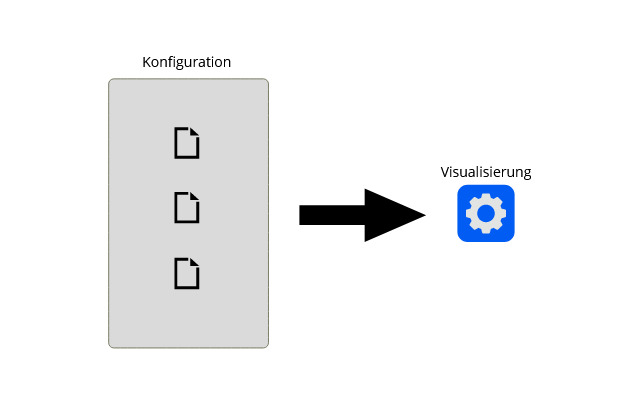
\includegraphics[width=\textwidth]{struktur_entwurf_1.jpg}
    \end{center}
\end{frame}

\begin{frame}{Probleme}
    \begin{itemize}
        \item Benötigt Kenntnisse in mehrere Bereiche
        \item Am Konfigurationsschema gebunden
        \item Konfiguration muss immer verarbeitet werden
    \end{itemize}
\end{frame}

\begin{frame}{Projektstruktur}
    \begin{center}
        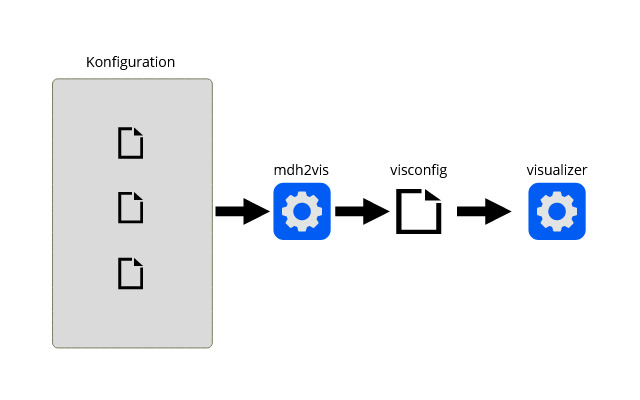
\includegraphics[width=\textwidth]{struktur_entwurf_2.jpg}
    \end{center}
\end{frame}

\begin{frame}{Projektstruktur}
    \begin{itemize}
        \item Unterteilung in mehreren Projekten
            \begin{itemize}
                \item mdh2vis
                \item visconfig
                \item visualizer
            \end{itemize}

        \item mdh2vis: Verarbeitet die MDH-Konfiguration
        \item visconfig: Spezifikation der Konfiguration des Visualisierungstool
        \item visualizer: Visualisierungstool
    \end{itemize}
\end{frame}

\begin{frame}{Projekt: visualizer}
    \begin{itemize}
        \item Aufgabe: Visualisierung und Simulation
        \item Grafikschnittstelle: OpenGL
        \item Sprache: C++
    \end{itemize}
\end{frame}

\begin{frame}{Projekt: visualizer}
    \begin{center}
        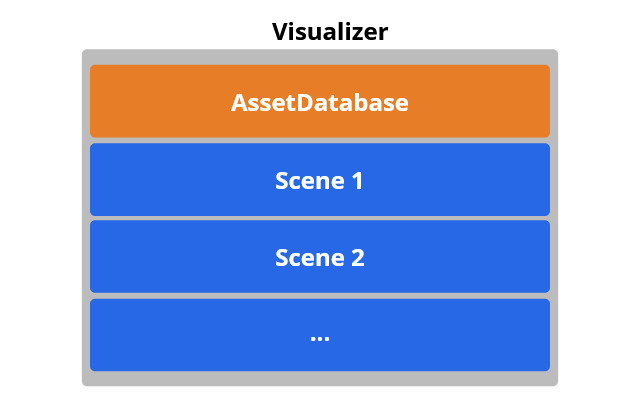
\includegraphics[width=\textwidth]{visualizer_structure.jpg}
    \end{center}
\end{frame}

\begin{frame}{Projekt: visualizer}
    \begin{itemize}
        \item AssetDatabase: Globale Ressourcen
        \item Scene: Zustand der Simulation
        \item Designprinzipien
        \begin{itemize}
            \item Render loop
            \item Data-oriented
            \item ECS (Entity-Component-System)
        \end{itemize}
    \end{itemize}
\end{frame}

\begin{frame}{ECS}
    \begin{itemize}
        \item Mehrere Welten pro Scene
        \item Welt: Isolierte Menge von Daten und Operationen
        \begin{itemize}
            \item Entity: Logische Gruppierung von Daten
            \item Component: Daten
            \item System: Operationen
        \end{itemize}
    \end{itemize}
\end{frame}

\begin{frame}{World}
    \begin{center}
        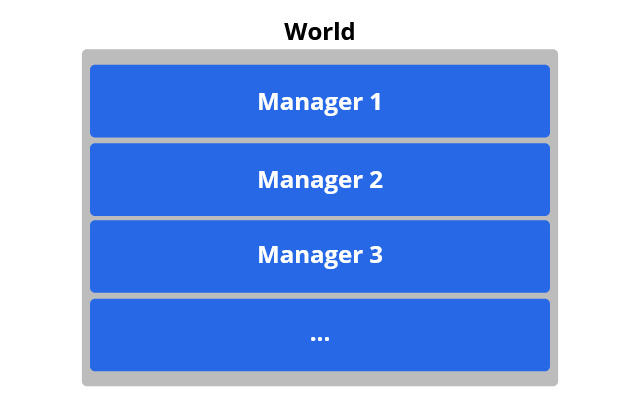
\includegraphics[width=\textwidth]{world_structure_general.jpg}
    \end{center}
\end{frame}

\begin{frame}{World}
    \begin{center}
        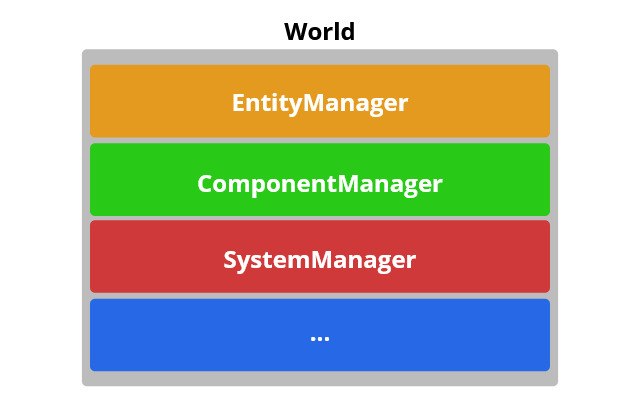
\includegraphics[width=\textwidth]{world_structure_specific.jpg}
    \end{center}
\end{frame}

\begin{frame}{ECS}
    \begin{itemize}
        \item EntityManager: Erzeugt/Entfernt Entitäten
        \item ComponentManager: Enthält alle Komponenten
        \item SystemManager: Enthält alle Operationen
    \end{itemize}
\end{frame}

\begin{frame}{Archetype}
    \begin{center}
        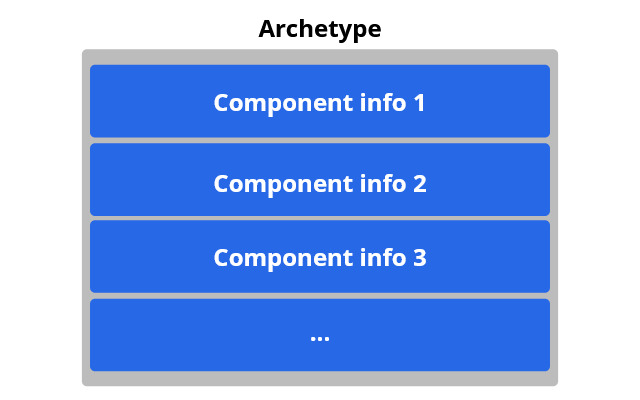
\includegraphics[width=\textwidth]{archetype.jpg}
    \end{center}
\end{frame}

\begin{frame}{ComponentMap}
    \begin{center}
        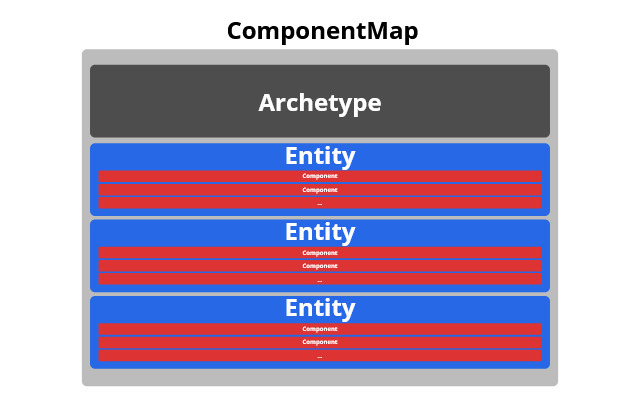
\includegraphics[width=\textwidth]{componentmap.jpg}
    \end{center}
\end{frame}

\begin{frame}{ComponentMap}
    \begin{itemize}
        \item Jede Entität gehört zu genau einer ComponentMap
        \item Alle Entitäten in einer ComponentMap haben dieselbe Struktur
        \item Archetype beschreibt die Struktur
    \end{itemize}
\end{frame}

\begin{frame}{SystemManager}
    \begin{center}
        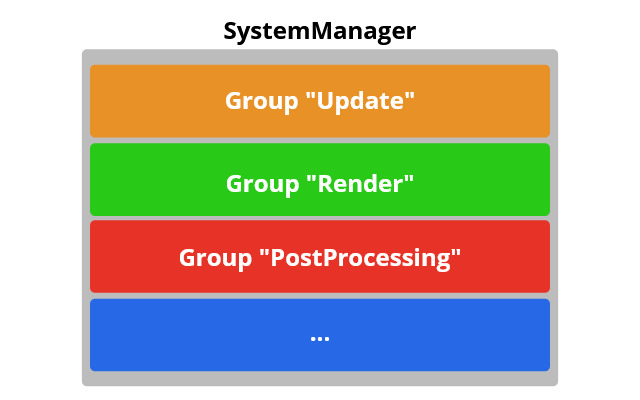
\includegraphics[width=\textwidth]{systemmanager_structure.jpg}
    \end{center}
\end{frame}

\begin{frame}{Group}
    \begin{center}
        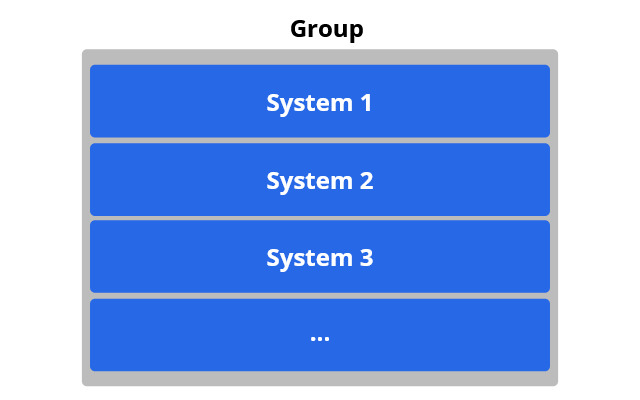
\includegraphics[width=\textwidth]{group_structure.jpg}
    \end{center}
\end{frame}

\begin{frame}{Group}
    \begin{itemize}
        \item Alle Systeme in einer Gruppe werden nacheinander ausgeführt
        \item Gruppen können einzeln ausgeführt werden
        \item Ermöglicht Abhängigkeiten von Operationen zu Modellieren
    \end{itemize}
\end{frame}

\begin{frame}{Vorteile}
    \begin{itemize}
        \item \textbf{„Wenn es aussieht wie eine Ente, 
                        schwimmt wie eine Ente und quakt wie eine Ente, 
                        dann ist es wahrscheinlich eine Ente.“ }
        \item Entitäten sind nicht interessant
        \item Komponenten sind viel wichtiger
        \item Komposition vs. Vererbung
    \end{itemize}
\end{frame}

\begin{frame}{Beispiel: Allgemein}
    \begin{itemize}
        \item Ann:
        \begin{itemize}
            \item Ent: Menge aller Entitäten
            \item Komp: Menge aller Komponenten
            \item $Q \subseteq \text{Ent}$: Query
            \item $C_1,C_2,...,C_n \in \text{Komp}$: Gesuchte Komponente
            \item $C_{n+1},C_{n+2},...,C_m \in \text{Komp}$: Verworfene Komponente
        \end{itemize}
        \item $Q := \{ E \in \text{Ent} | C_i \in E \wedge C_j \notin E, \forall i \in \{1,...,n\}, j \in \{n+1,...,m\}\}$
    \end{itemize}
\end{frame}

\begin{frame}{Beispiel: Kamera}
    \begin{itemize}
        \item Kann aktiv sein
        \item Kann sich frei bewegen (WASD + Mouse)
        \item Dreht sich um einen Punkt
    \end{itemize}
\end{frame}

\begin{frame}{Beispiel: Kamera}
    \begin{itemize}
        \item Object-oriented:
        \begin{itemize}
            \item Superklasse: Camera
            \item FreeCamera (erbt von Camera)
            \item FixedCamera (erbt von Camera)
        \end{itemize}
        \item Data-oriented:
        \begin{itemize}
            \item Camera
            \item FreeCamera
            \item FixedCamera
            \item CameraRenderingSystem
            \item FreeCameraMovementSystem
            \item FixedCameraMovementSystem
        \end{itemize}
    \end{itemize}
\end{frame}

\begin{frame}{Beispiel: Kamera}
    \begin{itemize}
        \item Suche alle Kameras (Formal)
        \item Ann:
        \begin{itemize}
            \item Ent: Menge aller Entitäten
            \item $Q \subseteq \text{Ent}$: Menge aller Kameras
        \end{itemize}
        \item $Q := \{ E \in \text{Ent} | \text{Camera} \in E \wedge (\text{FreeCamera} \in E \vee \text{FixedCamera} \in E)\}$
    \end{itemize}
\end{frame}

\begin{frame}{Beispiel: Kamera}
    \begin{itemize}
        \item Suche alle Kameras (Formal)
        \item Ann:
        \begin{itemize}
            \item Ent: Menge aller Entitäten
            \item $Q \subseteq \text{Ent}$: Menge aller Kameras
        \end{itemize}
        \item $Q := \{ E \in \text{Ent} | \text{Camera} \in E \wedge (\text{FreeCamera} \in E \vee \text{FixedCamera} \in E)\}$
    \end{itemize}
\end{frame}

\begin{frame}{Beispiel: Kamera}
    \begin{center}
        \lstinputlisting[style=context,xleftmargin=2em]{camera_query.cpp}
    \end{center}
\end{frame}

\begin{frame}{Komponenten}
    \begin{itemize}
        \item Camera
        \item FreeFlyCamera
        \item FixedCamera
        \item Iteration
        \item Cube
        \item Material
        \item Mesh
        \item ...
    \end{itemize}
\end{frame}

\begin{frame}{Komponenten}
    \begin{itemize}
        \item Identifikatoren: Leere Strukturen
        \begin{itemize}
            \item Cube
            \item FreeFlyCamera
            \item ...
        \end{itemize}
        \item Zweck spezifisch: Nicht leere Strukturen
        \begin{itemize}
            \item Camera
            \item Material
            \item Mesh
            \item ...
        \end{itemize}
    \end{itemize}
\end{frame}

\begin{frame}{Systeme}
    \begin{itemize}
        \item Gruppen:
        \begin{itemize}
            \item Update: Simulation
            \item Render: Zeichnet die Szene
            \item PostProcessing: Bringt die Bilder auf den Bildschirm
        \end{itemize}
        \item Systeme:
        \begin{itemize}
            \item CubeMovementSystem
            \item FreeFlyCameraMovementSystem
            \item FixedCameraMovementSystem
            \item MeshDrawingSystem
            \item CompositingSystem
            \item ...
        \end{itemize}
    \end{itemize}
\end{frame}

\end{document}

% vi: tw=100
